\chapter{Methodology}
\label{chapter:methodology}

\begin{introduction}
"The things we lose have a way of coming back to us in the end,

if not always in the way we expect"

- J.K. Rowling, Harry Potter and the Order of the Phoenix (2003)
\end{introduction}

This section begins by defining the phases that constitute the research. Following that, it outlines the beginning of the design of the system's structure by defining its architecture, features, and workflows. To meet the acceptance criteria for this stage and take into account the volume of this research, a strategic framework was selected to guide the architectural design of the proposed solution. By leveraging the principles and steps of \ac{acdm}, this chapter defines the solution's initial requirements, stakeholders, challenges and architecture.

% ____________________ Phases of the Research ____________________ %

\section{Phases of the Research} \label{section:phases_of_the_research}

To realise the previously mentioned objectives, the proposed research can be conducted in four key stages, which align with a logical progression from understanding the problem to focusing on different aspects of design and development.

\begin{outline}[enumerate]
    \1 Study the State-of-the-Art and identify design approaches:
        \2 Review existing ;
        \2 \aclp{lfms};
        \2 In-production solutions;
        \2 Available and recommended technologies;
        \2 Best practices and optimal approaches;
    \1 Design the structure of the system by defining its architecture, features and workflows;
    \1 Create the main system components, including all the planned features;
    \1 Test the system in a real-world and controlled environment;
    \1 Finalise and document the results for academic and practical use.
\end{outline}

% ____________________ Architecture-Centric Development Methodology ____________________ %

\section{\acl{acdm}} \label{section:acdm}

The \ac{acdm} is a software development methodology, mainly inspired by Quality Attribute Workshop, Architecture Tradeoff Analysis Method and Attribute Driven Design, that emphasises the use of software architecture as a primary driver for the development process \cite{Lattanze2005}. It integrates architectural design into the overall lifecycle of software development, aiming to improve quality, predictability, and efficiency. Below are the key aspects of \ac{acdm} based on the provided paper. \ac{acdm} is structured around the concept that software architecture serves as the backbone of the system, providing a framework for ensuring consistency, scalability, and alignment with business goals. The architecture is not only a technical construct but also a means of communication among stakeholders.

% ____________________ Definition ____________________ %

\subsection{Definition}

As shown in Figure \ref{fig:acdm_workflow}, the \ac{acdm} organises the architectural design process into clearly defined stages that evolve iteratively. \ac{acdm} is inherently iterative, with the flexibility to revisit earlier stages based on findings or changing requirements.

\begin{figure}[!htb]
    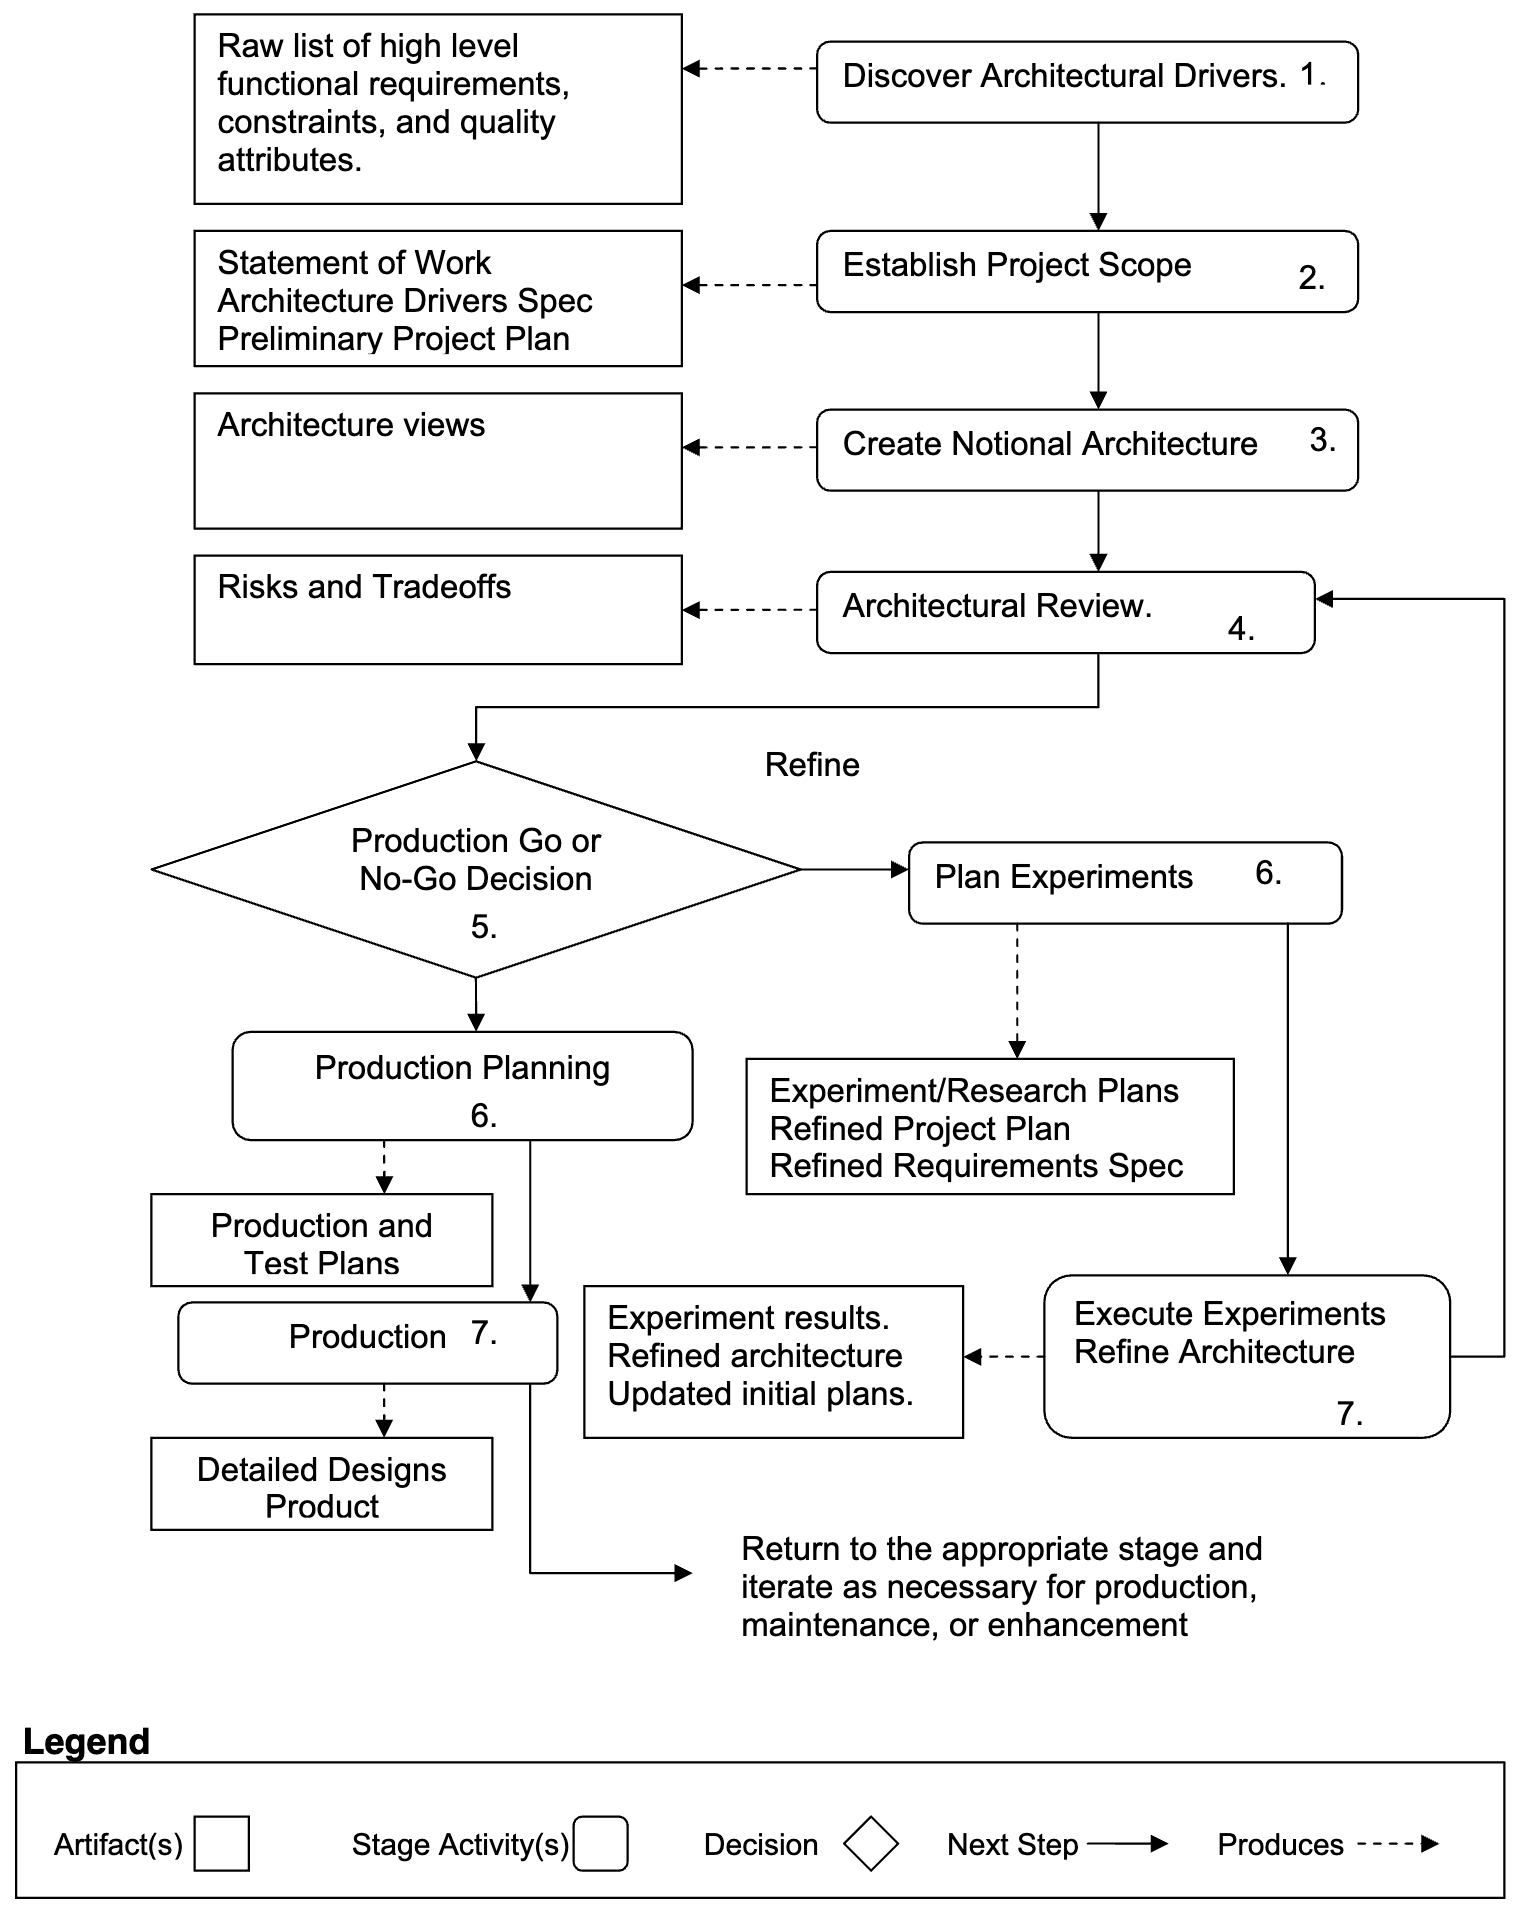
\includegraphics[width=0.6\textwidth]{figs/chapter3/acdm_workflow.png}
    \centering
    \caption[\acl{acdm} Workflow]{\ac{acdm} workflow, illustrating the iterative stages, the flow of artifacts, decisions, and refinements through the development process. Adapted from \citeauthoryear{Lattanze2005}.}
    \label{fig:acdm_workflow}
\end{figure}

\subsubsection{Architectural Drivers}

According to \citeauthoryear{Lattanze2005}, the process begins with discovering the architectural drivers, where crucial factors such as functional requirements, quality attributes (e.g., performance, scalability, security), and constraints are identified. These drivers form the foundation for all subsequent design decisions. Appendix \ref{app:architectural-design} contains the remaining stages of the \ac{acdm} process, which provide a fully defined set of the architectural drivers for this research.

\subsubsection{Project Scope}

Following this, the project scope is established to define the system's boundaries, objectives, deliverables, and constraints, ensuring that all stakeholders have a shared understanding of the project's limits and expectations.

\subsubsection{Notional Architecture}

Once the drivers and scope are defined, a notional architecture is created as a high-level conceptual design. This step involves decomposing the system into components, defining their responsibilities, interactions, and dependencies, and adopting appropriate architectural styles and patterns. The notional architecture serves as a blueprint for early-stage validation.

\subsubsection{Architectural Review}

The design is then subjected to an architectural review, where it is assessed against the architectural drivers and project scope. Scenario-based evaluations, risk assessments, and stakeholder feedback are key activities during this stage. The outcome is a decision to either proceed to production or refine the architecture further.

\subsubsection{Refinement Phase}

If the architecture is deemed insufficient during the review, the process enters a refinement phase. This phase begins with the \textbf{experiment planning}, where targeted experiments are designed to address specific weaknesses or uncertainties, such as performance bottlenecks or scalability challenges. These experiments are executed in the \textbf{experiment execution} and subsequent \textbf{architecture refinement} stage, with findings informing updates to the architecture. Once refined, the updated architecture undergoes another review to ensure it meets the required standards before moving forward.

\subsubsection{Production Phase}

If the architecture passes the review, the process transitions to the production phase, beginning with the \textbf{production planning}, which involves preparing the system for deployment by developing detailed plans, establishing monitoring mechanisms, and guaranteeing operational readiness. Finally, the system is deployed during the \textbf{production} stage, when it becomes operational and accessible to end-users. Post-deployment, the architecture is continuously monitored for performance and feedback, allowing iterative improvements as needed.

% ____________________ Quality Attributes ____________________ %

\subsection{Quality Attributes} \label{section:quality_attributes}

The quality attributes serve as a foundation for developing the platform. The selection of the following attributes was guided by their crucial role in guaranteeing the solution's success and addressing the key challenges identified in the problem domain.

The following quality attributes were selected based on their priority to the solution's success and the challenges identified in the problem domain.

\subsubsection{Scalability}

The platform must accommodate a growing user base and increased item-tracking demands across diverse locations. A microservices architecture is proposed to enable independent scaling of critical system components, such as user management and item management. This scalability aligns with the goal of creating a community-oriented system capable of handling high-traffic scenarios and fluctuations in demand without compromising performance.

\subsubsection{Reliability} 

Consistent performance is essential, even in adverse conditions like network failures. Ensuring reliability contributes to promoting user trust, a cornerstone of a lost property management system, aiming to build credibility among stakeholders. Fault-tolerant mechanisms, such as distributed databases and redundant servers, will be integrated to secure high availability (targeting 99\% uptime) and minimise the "mean time to repair"\footnote{\url{https://www.atlassian.com/incident-management/kpis/common-metrics}}. Automated monitoring and self-healing protocols will detect and address faults proactively.

\subsubsection{Security}

Handling sensitive data, such as user information and potentially high-value lost items, requires a security-first approach. Security measures further reinforce the platform's reliability and address concerns like identity theft and elevated access, two key pain points identified in this research. End-to-end encryption for secure authentication and granular authorisation mechanisms will protect data privacy. Due to the sensitivity of the data the system is going to handle, it is obliged to adhere to \ac{gdpr}\footnote{\url{https://gdpr-info.eu/}} and other relevant regulations to ensure the lawful handling of personal information.

\subsubsection{Usability}

The system targets a broad spectrum of users, including non-technical individuals, necessitating an intuitive and accessible interface. Implementing \ac{ui} and \ac{ux} best practices and ongoing feedback loops will promote an iterative improvement of the platform's interface. Multilingual support and visual guidance will also cater to diverse user demographics.

\subsubsection{Observability}

Incorporating observability tools to collect logs, metrics, and traces will allow real-time and long-term monitoring of the system's performance and user interactions. Observability also allows quick detection and resolution of operational issues, providing insights for continuous improvement.

% ____________________ Requirements ____________________ %

\subsection{System Requirements} \label{section:requirements}

The system's design and implementation are guided by its requirements, which can also be used to measure the research progress and value. When correctly specified, they help the developer understand the expected result, and the stakeholders evaluate the system's performance. These requirements are divided into two categories: functional and non-functional. Table \ref{tab:functional_requirements} lists the functional requirements that define the core features of the system, focusing on enabling users to interact with and manage data effectively.

\begin{table}[!htb]
\centering
\begin{tabular}{|p{0.1\textwidth}|p{0.80\textwidth}|}
\hline
\textbf{ID} & \textbf{Functional Requirement Description} \\ \hline
FR1 & Support three user roles: ordinary users, local managers, and administrators. \\ \hline
FR2 & Enable secure account management for all user types. \\ \hline
FR3 & Implement authentication and authorization mechanisms, including multi-factor authentication. \\ \hline
FR4 & Allow users to browse and search lost items based on categories and filters (e.g., location, type). \\ \hline
FR5 & Provide personalized suggestions for matching items using \ac{ai}. \\ \hline
FR6 & Facilitate item status updates and notifications to users about item matches or updates. \\ \hline
FR7 & Enable users to schedule appointments for item retrieval. \\ \hline
FR8 & Allow administrators to audit system logs and manage user roles effectively. \\ \hline
FR9 & Integrate community-driven features for collaborative lost item recovery. \\ \hline
\end{tabular}
\caption[Functional Requirements]{Functional requirements defining the core system features.}
\label{tab:functional_requirements}
\end{table}

On the other hand, Table \ref{tab:nonfunctional_requirements} presents the non-functional requirements, which are directly connected with the system's expected quality levels.

\begin{table}[!htb]
\centering
\begin{tabular}{|p{0.1\textwidth}|p{0.80\textwidth}|}
\hline
\textbf{ID} & \textbf{Non-Functional Requirement Description} \\ \hline
NFR1 & Ensure a response time of less than 2 seconds for critical operations under peak load. \\ \hline
NFR2 & Support scalability to accommodate up to 10,000 concurrent users. \\ \hline
NFR3 & Comply with data privacy regulations such as \ac{gdpr}. \\ \hline
NFR4 & Maintain 99\% uptime through fault tolerance and disaster recovery mechanisms. \\ \hline
NFR5 & Adhere to \ac{ux} and \ac{ui} best practices. \\ \hline
NFR6 & Implement modular and maintainable architecture for easier updates and debugging. \\ \hline
NFR7 & Incorporate monitoring tools for real-time performance tracking and troubleshooting. \\ \hline
NFR8 & Secure compatibility across devices. \\ \hline
\end{tabular}
\caption[Non-Functional Requirements]{Non-functional requirements defining the system's quality attributes.}
\label{tab:nonfunctional_requirements}
\end{table}


% ____________________ Constraints ____________________ %

\subsection{Constraints} \label{section:constraints}

The development of the system is governed by two primary constraints that shape its scope, deliverables, and quality:

\subsubsection{C1: Timeframe Limitation}

The development is restricted to a 10-month timeframe in which it is embedded.

\subsubsection{C2: Verifiable Quality}

Both software and design quality must be verifiable, meaning the stakeholders must test the system and review its code.

% ____________________ Notional Architecture ____________________ %

\subsection{Notional Architecture} \label{section:notional_architecture}

The proposed architecture, visible in Figure \ref{fig:notional_arch}, is designed as a microservices-based system, i.e., it divides the application into distinct, independent services, each responsible for a specific functionality. It is possible to group the architecture's components into three main layers: the frontend, backend, and support infrastructure, as follows:

\begin{figure}[!htb]
    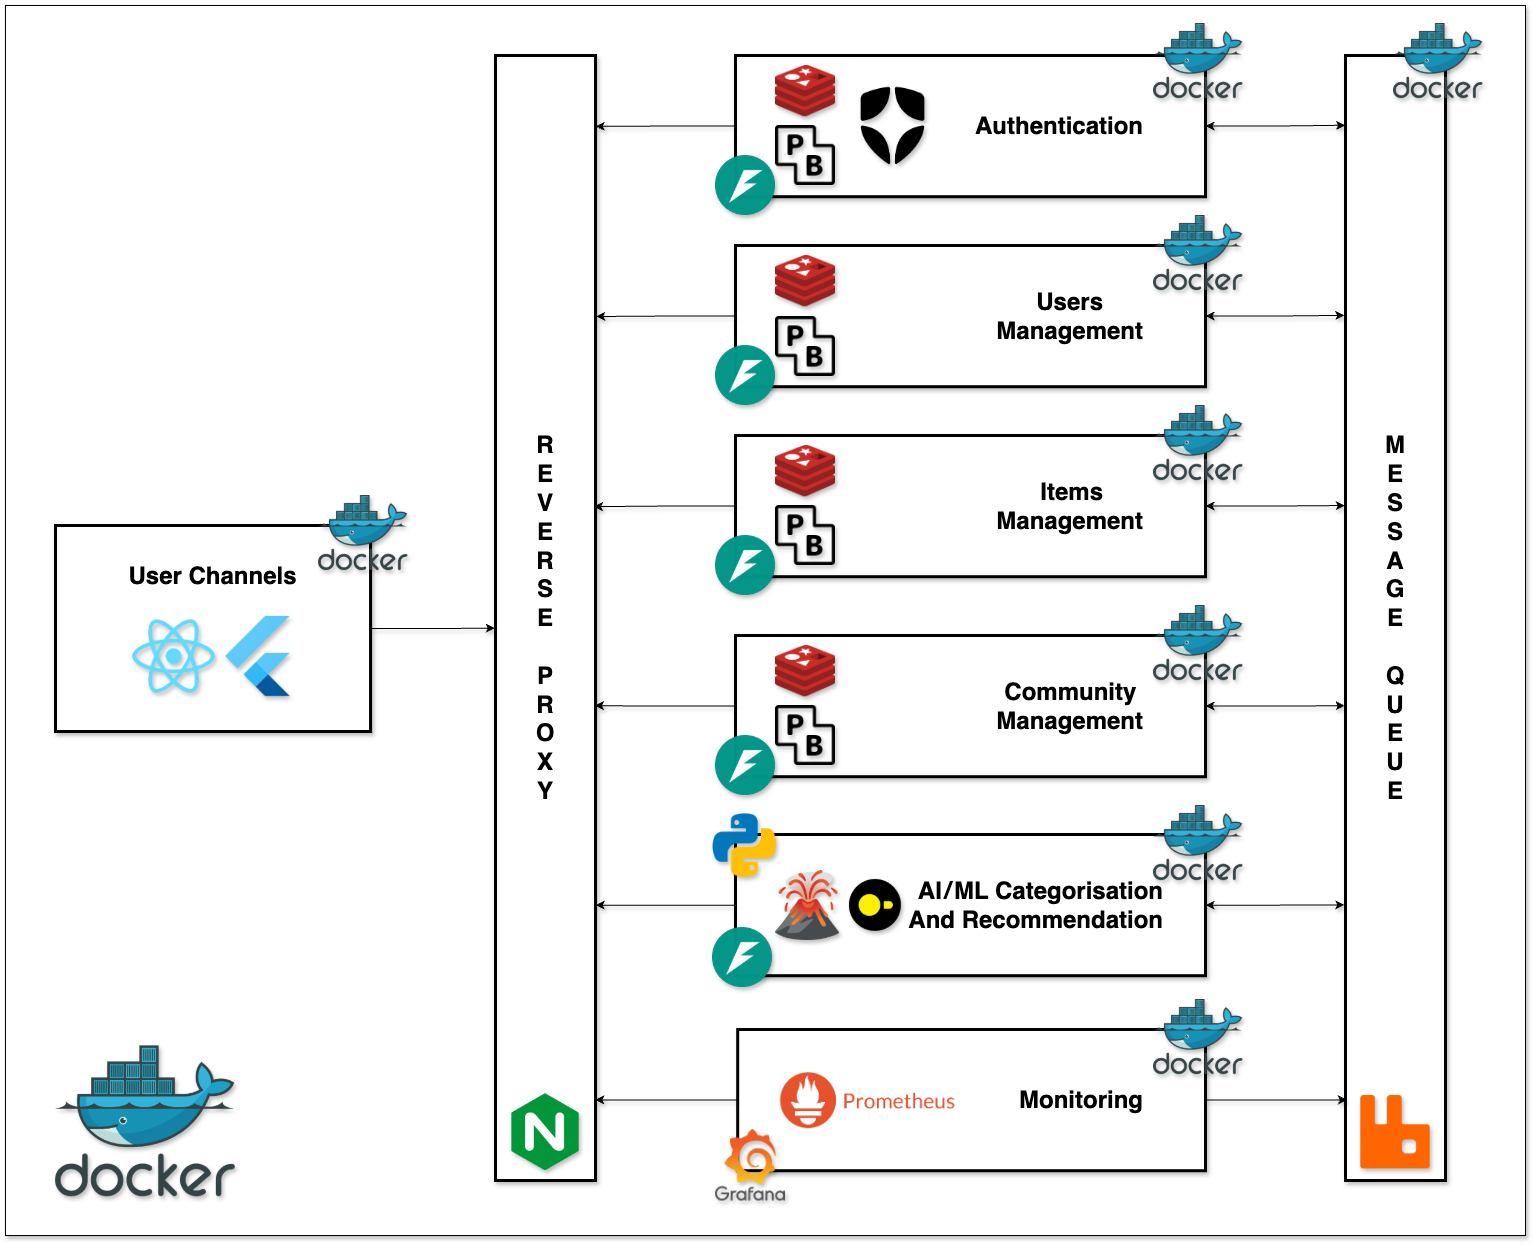
\includegraphics[width=0.8\textwidth]{figs/chapter3/notional_arch.png}
    \centering
    \caption[Notional Architecture]{High Level View of the First Iteration of the Notional Architecture.}
    \label{fig:notional_arch}
\end{figure}

\subsubsection{Frontend}

The frontend provides users with a seamless and intuitive interface for both web and mobile platforms, enabling easy access to all system features and smooth interaction with the backend services.

\subsubsection{Backend}

The backend is the core of the system and is structured as a collection of microservices that include:

\begin{itemize}
    \item Authentication Service: Through the use of role-based access control, it handles user authentication and authorisation, securing controlled access to the system;
    \item Users Management Service: Manages user profiles, including registration and updates;
    \item Items Management Service: The most likely core service of the system focuses on fetching, storing and updating lost items. It integrates with other services to provide seamless item tracking and retrieval functionalities;
    \item Community Management Service: Handles the direct communication between ordinary users and the chat spaces available for each community;
    \item \ac{ai}/\ac{ml} Categorization and Recommendation Service: Automatically identifies and categorises items based on images and descriptions. Processes user inputs and interactions to actively match and recommend items to ordinary users who search for an item.
\end{itemize}

\subsubsection{Support Infrastructure}

The infrastructure provides the foundation for deploying and managing the system. It includes the following key components:

\begin{itemize}
    \item Reverse Proxy: Routes incoming requests to the appropriate services. It also provides load balancing and enhances the system's overall security by handling HTTPS termination;
    \item Message Queue: Facilitates asynchronous communication between microservices to ensure that each service operates independently, even during high data throughput;
    \item Monitoring: Collects performance metrics and provides a dashboard for real-time visualisation.
\end{itemize}

% ____________________ Technology Stack ____________________ %

\subsubsection{Proposed Technologies to be Used}

The selection of technologies is based on their alignment with the architectural drivers and the system's requirements. The proposed technology stack is as follows:

For the frontend, React\footnote{\url{https://react.dev/}} will be used to build a dynamic and interactive web application, mainly for administrative uses inside the platform. At the same time, Flutter will enable cross-platform mobile application development, ensuring an accessible and consistent user experience across locations and devices.

The backend will be essentially powered by FastAPI\footnote{\url{https://fastapi.tiangolo.com/}}, a Python\footnote{\url{https://www.python.org/}}-based framework that excels at building high-performance \acp{api} for small/medium projects, which main propose is supporting asynchronous operations. Authentication will be secured using OAuth 2.0\footnote{\url{https://oauth.net/2/}}, a widely adopted protocol, that will capable of granting and managing secure access and role-based access control. The system will rely on Pocketbase\footnote{\url{https://pocketbase.io/}}, an open-source Backend-as-a-Service, for handling database operations, real-time data sync, complemented by Redis\footnote{\url{https://redis.io/}} for caching and session management, in order to guarantee a fast data access and reduce the backend load. For \ac{ai}-driven functionalities, \ac{llava}\footnote{\url{https://llava-vl.github.io/}}, an end-to-end trained large multimodal, will combine language and vision processing. Data analytics will be supported by DuckDB\footnote{\url{https://duckdb.org/}}, an in-process analytical database that efficiently processes the complex embeddings generated by \ac{llava}. Considering the necessity of valuable monitoring, Prometheus\footnote{\url{https://prometheus.io/}} will collect metrics across the system, and, using Grafana\footnote{\url{https://grafana.com/}}, it will ale to have intuitive dashboards for real-time visualisation and performance tracking. 

The entire infrastructure will be containerised using Docker\footnote{\url{https://www.docker.com/}}, ensuring consistency across environments and simplifying deployment. Nginx\footnote{\url{https://nginx.org/en/}} will act as a reverse proxy and load balancer, enhancing request routing. Finally, RabbitMQ\footnote{\url{https://www.rabbitmq.com/}} will serve as the unique message broker, enabling asynchronous and reliable communication between the microservices.

% ____________________ Future Work and Work Plan ____________________ %

\section{Future Work and Work Plan} \label{section:future_work_and_work_plan}

The next phase involves the implementation of the proposed architecture, starting by creating a \ac{mvp} to test the initial functionalities. The \ac{mvp} will focus on the item management service, user registration and authentication, and the community management service. The \ac{mvp} will be iteratively refined based on user feedback and performance metrics, ensuring that the system meets the acceptance criteria defined in this research. This \ac{mvp} will integrate most of the \ac{ims} features and is expected to be a full \ac{lfms}, capable of handling lost items and user interactions. The \ac{ai}/\ac{ml} categorisation and recommendation service will be developed in parallel to the \ac{mvp} testing and will be integrated into the system once it reaches a stable state, resulting from the feedback and improvements made. Once the service responsible for the system's intelligence is integrated, the system will, once again, be tested and refined to guarantee that the functionalities are working as expected and that the system meets the acceptance criteria and fulfils the architectural drivers and the dissertation's objectives.

The dissertation document will be continuously updated throughout the system's development to reflect the progress made. It will also include the system's testing results and the feedback received from users and stakeholders. The final version of the document will include a detailed analysis of the system's performance and usability, as well as a discussion of the lessons learned and the potential for future research.

Figure \ref{fig:gantt_diagram} illustrates the work plan for the next phase, outlining the key activities and milestones to be achieved.

\begin{figure}[!htb]
    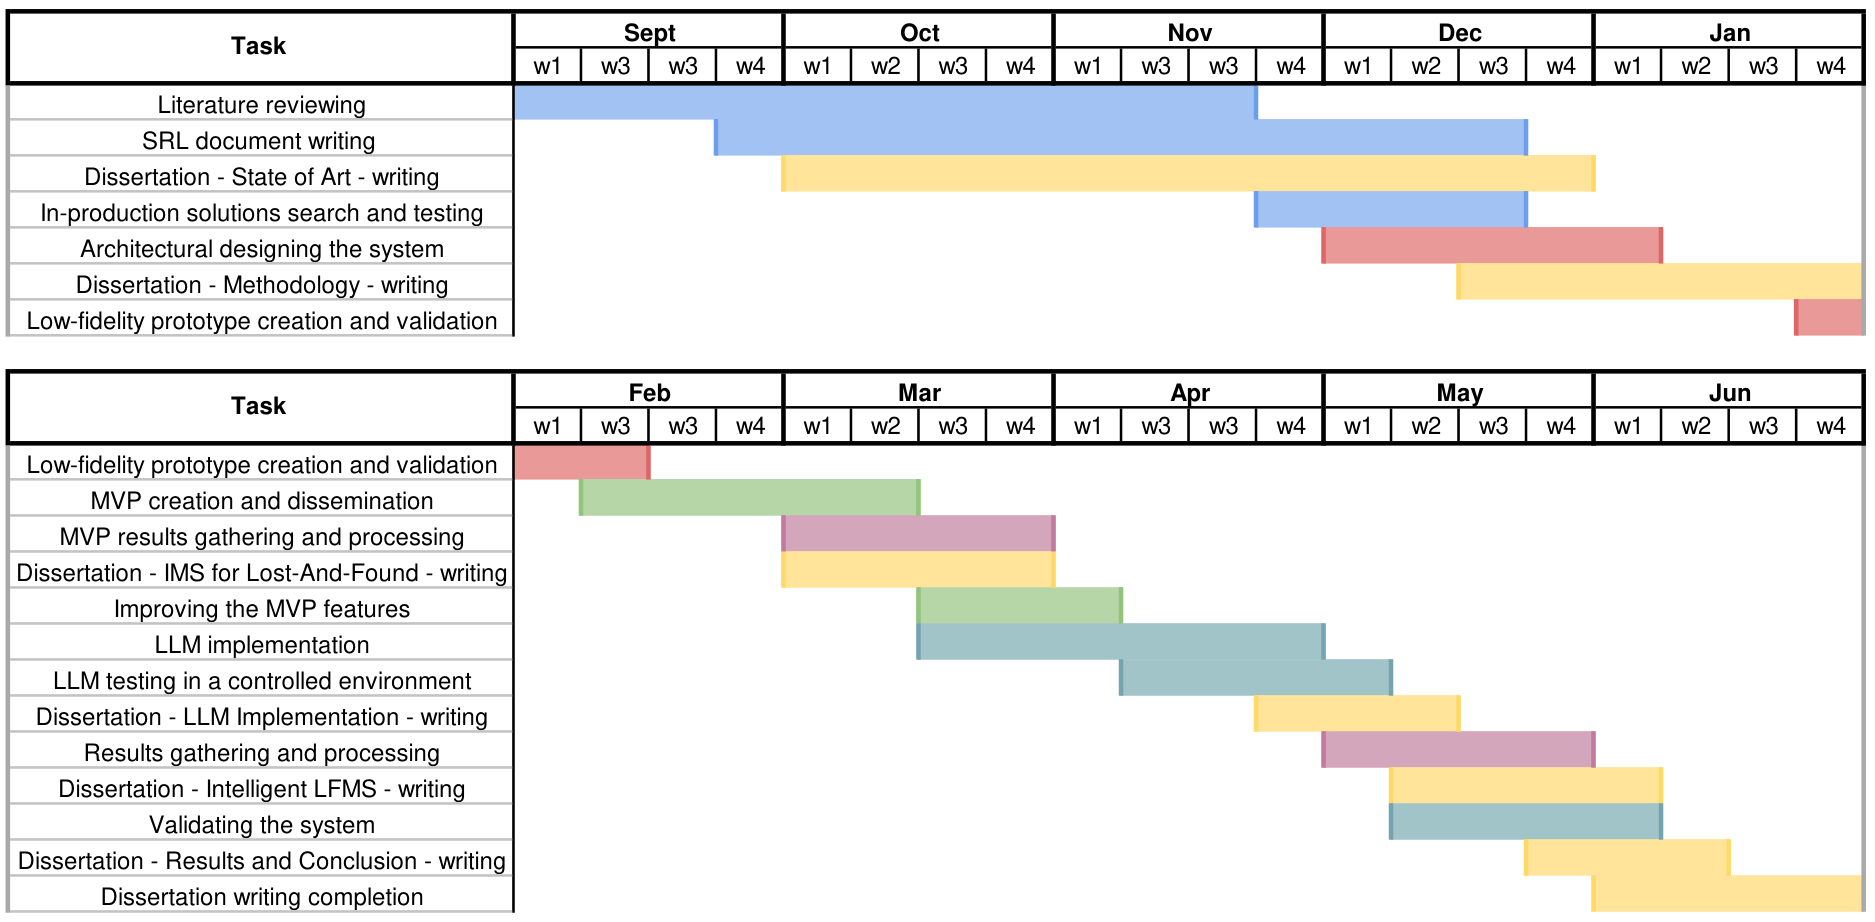
\includegraphics[width=0.95\textwidth]{figs/chapter3/gantt_diagram.png}
    \centering
    \caption[Expected dissertation's work plan expressed in a Gantt diagram]{Expected dissertation's work plan expressed in a Gantt diagram.}
    \label{fig:gantt_diagram}
\end{figure}

% \section{Study Case} \label{section:case_study}

% TODO: Write this section

% \section{Work Environment} \label{section:work_environment}

% TODO: Write this section

% \section{Summary} \label{section:chapter3_summary}

% TODO: Write this section